\subsection{Decentralized SGF FW Experiments}
To study the performance of Algorithm \ref{decentralized} we considered a portion of the MNIST test set made of 1000 samples. Each of the $M=10$ workers received 100 images, 10 for each class.
We then tuned the hyperparameter $m$ for the number of directions to be sampled in the I-RDSA scheme. The best value for which the lowest accuracy (approximatively 20\%) of LeNet-5 was reached is $m=35$, as shown in Figure \ref{fig:accuracy}.\\
\begin{figure}[htbp]
	\centering
	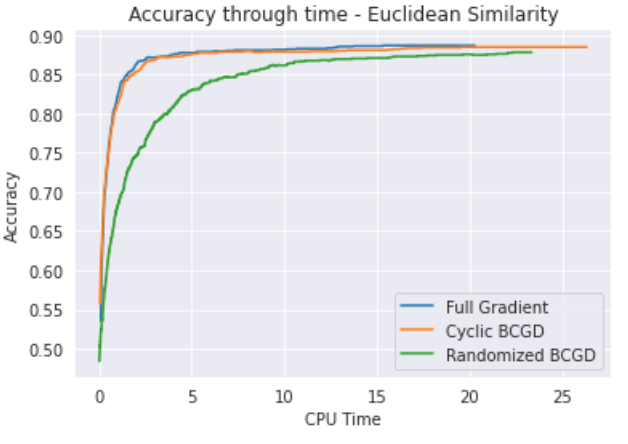
\includegraphics[width=6cm]{accuracy.png}
	\caption{{\small This plot was obtained by running Algorithm \ref{decentralized} multiple times, while changing the value of the parameter $m$ (horizontal axis) from $5$ to $40$ by keeping all the other parameter fixed. The vertical axes indicates the values of the accuracy.}}
	\label{fig:accuracy}
\end{figure}
\indent With the increasing of $m$, the running time becomes very large and for this reason we had to find a value for $m$ which returns a low accuracy with respect to a reasonable running time. We ended up with $m=15$, which is a good compromise between the previous ones, and we kept this value fixed for all the runs.\\
\indent In particular, we performed three different experiments, considering $T=20$, $T=50$ and $T=100$. As the number of queries increases, the pattern of the perturbation becomes clearer, and in Figure \ref{fig:decentralized_perturbations} we can see how the 3-shape perturbation becomes more evident for higher values of $T$. 
\begin{figure}[h]
	\centering
	\begin{subfigure}[b]{0.15\textwidth}
		\centering
		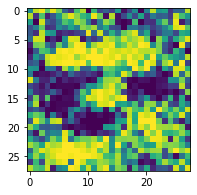
\includegraphics[width=2.3cm]{T20_final.png}
		\caption{}
		\label{fig:decentralized_perturbation_20}
	\end{subfigure}
	\hfill
	\begin{subfigure}[b]{0.15\textwidth}
		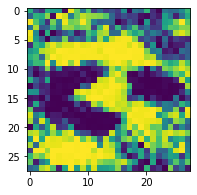
\includegraphics[width=2.3cm]{T50_final.png}
		\caption{}
		\label{fig:decentralized_perturbation_50}
	\end{subfigure}
	\hfill
	\begin{subfigure}[b]{0.15\textwidth}
		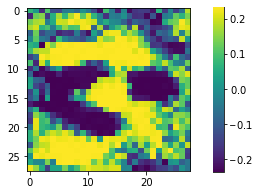
\includegraphics[width=3cm]{T100_bar.png}
		\caption{}
		\label{fig:decentralized_perturbation_100}
	\end{subfigure}
	\caption{{\small Perturbations generated by the Decentralized SGF FW algorithm with different numbers of queries: (a) T=20, (b) T=50, (c) T=100.}}
	\label{fig:decentralized_perturbations}
\end{figure}

This behaviour is coherent with the decreasing of the accuracy reported in Table \ref{tab:decentralized}: to a lower accuracy corresponds a sharper pattern in the perturbation.

It is interesting to notice that with $T=20$ queries of Algorithm \ref{decentralized} the accuracy of LeNet-5 already decreases to 55,25\%.
\begin{table}[htbp]
	\begin{center}
		\begin{adjustwidth}{-.6cm}{}
			\begin{tabular}{c|ccc}
				\textbf{Attack} &          20 \textbf{queries} &      50 \textbf{queries} &     100 \textbf{queries} \\
				\midrule
				{\small Decentralized SGF FW}     &    55,25\% &    39,46\% &       36,87\% \\
			\end{tabular}
		\end{adjustwidth}
	\end{center}
	\caption{{\small  Summary of $\ell_\infty$ Universal Adversarial Perturbation with $\varepsilon$=0.25. MNIST attacks using Decentralized SGF FW. The entries of the table represent the accuracies of LeNet-5 for the three different attacks.}}
	\label{tab:decentralized}
\end{table}

In Figure \ref{fig:decentralized} is represented the perturbation of Figure \ref{fig:decentralized_perturbations} (c)
applied on an image from class 4. The perturbed images have been classified as 3, consistently with the 3-shape of the perturbation.
\begin{figure}[htbp]
	\centering
	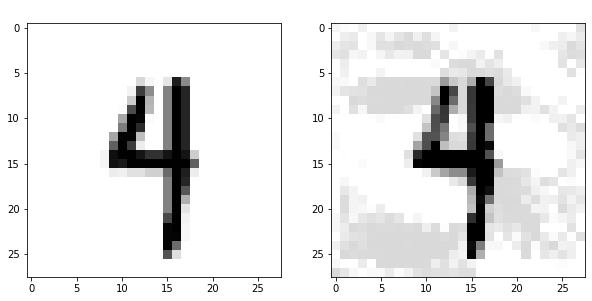
\includegraphics[width=6cm]{image_pertub_T100_final.png}
	\caption{{\small Image belonging to class 4 but classified as 3 by using the adversarial perturbation in Figure \ref{fig:decentralized_perturbations} (c) generated by the Decentralized SGF FW method.}}
	\label{fig:decentralized}
\end{figure}
\begin{figure}[htbp]
	\centering
	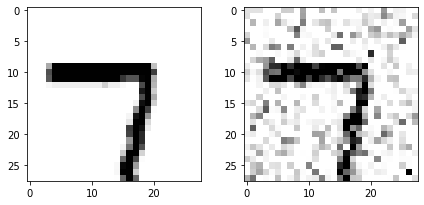
\includegraphics[width=6cm]{gaussian_image.png}
	\caption{{\small Image belonging to class 7 and correctly classified by the network despite the gaussian noise.}}
	\label{fig:gaussian_noise}
\end{figure}
To have a yardstick, the predictions of LeNet-5 remain very precise (89.17\% of accuracy) when tested on the images perturbed with random noise (Gaussian with mean 0 and standard deviation 0.3). Even though Figure \ref{fig:gaussian_noise} shows a very evident noise compared to the one of the adversarial example in the previous image, the network still classifies correctly the images perturbed with a Gaussian noise.

It is noteworthy the comparison between the attacks: the Gaussian perturbation spreads the noise randomly in the space, while the Decentralized SGF FW's adversarial perturbation is characterize by a clear pattern that covers the majority of the image space and allows to fool the network on most images.